\begin{frame}{Apron Foot}

\begin{figure}
\centering

\begin{subfigure}{0.48\textwidth}
    \centering
    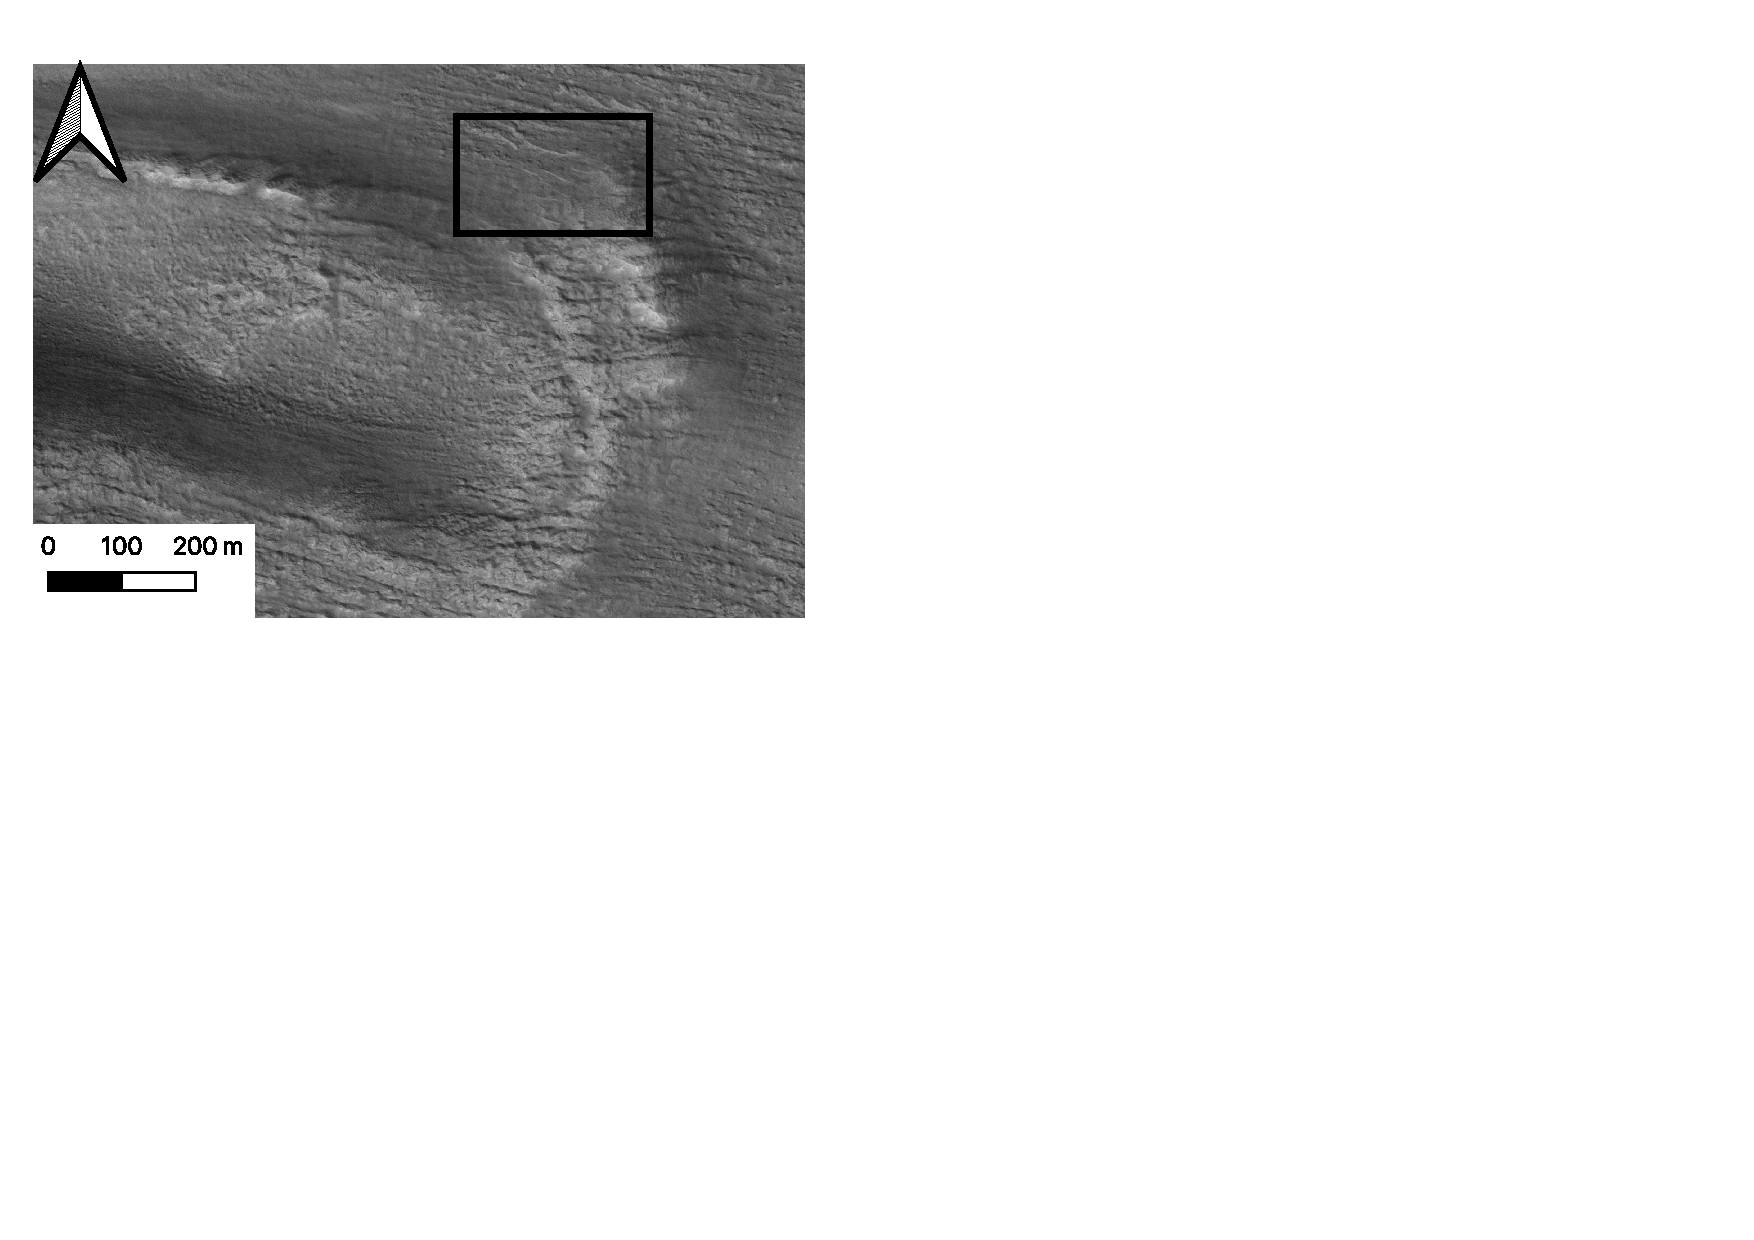
\includegraphics[
        width=\linewidth,
        height=0.65\textheight,
        keepaspectratio
    ]{Figures/HiRISE/Foot_Img.pdf}
    \label{fig:Foot_a}
\end{subfigure}
\hfill
\begin{subfigure}{0.48\textwidth}
    \centering
    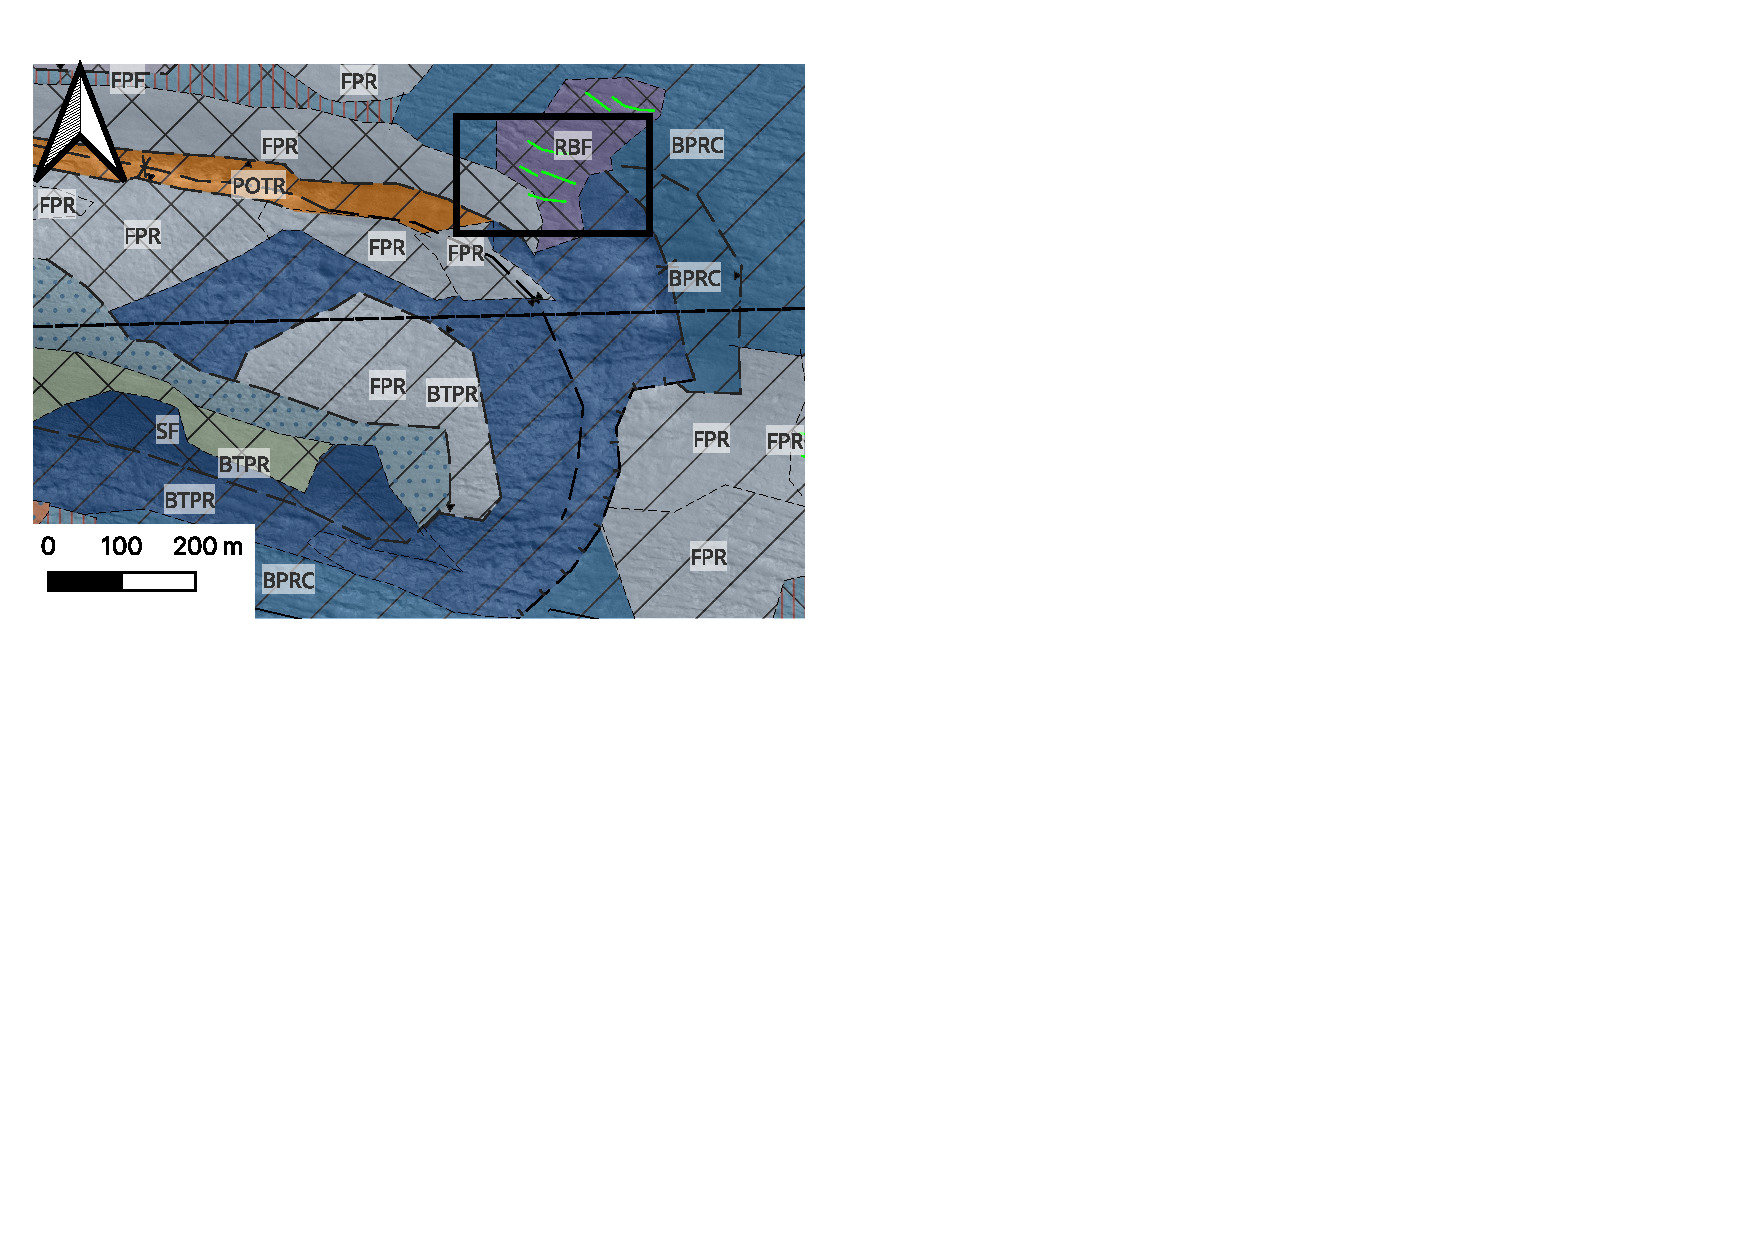
\includegraphics[
        width=\linewidth,
        height=0.65\textheight,
        keepaspectratio
    ]{Figures/HiRISE/Foot_Map.pdf}
    \label{fig:Foot_b}
\end{subfigure}

\caption{The apron foot. Note the rise and transverse-overprinted ridges (centred at $34.62301^{\circ}$N, $16.83755^{\circ}$E).}
\label{fig:Foot}
\end{figure}
\end{frame}
